% Start point: Porter model Author: Charles-Axel Dein URL: http://www.texample.net/tikz/examples/porter-model/
\documentclass[10pt,a4paper]{article} 

\usepackage[hmargin=1cm,vmargin=1.5cm]{geometry}
\renewcommand{\rmdefault}{bch} % change default font

\usepackage[english]{babel}
\usepackage[utf8]{inputenc}
\usepackage{tikz} 
\usetikzlibrary{arrows,decorations.pathmorphing,backgrounds,fit,positioning,shapes.symbols,chains}

\begin{document}

%\begin{figure}[h]
%\centering
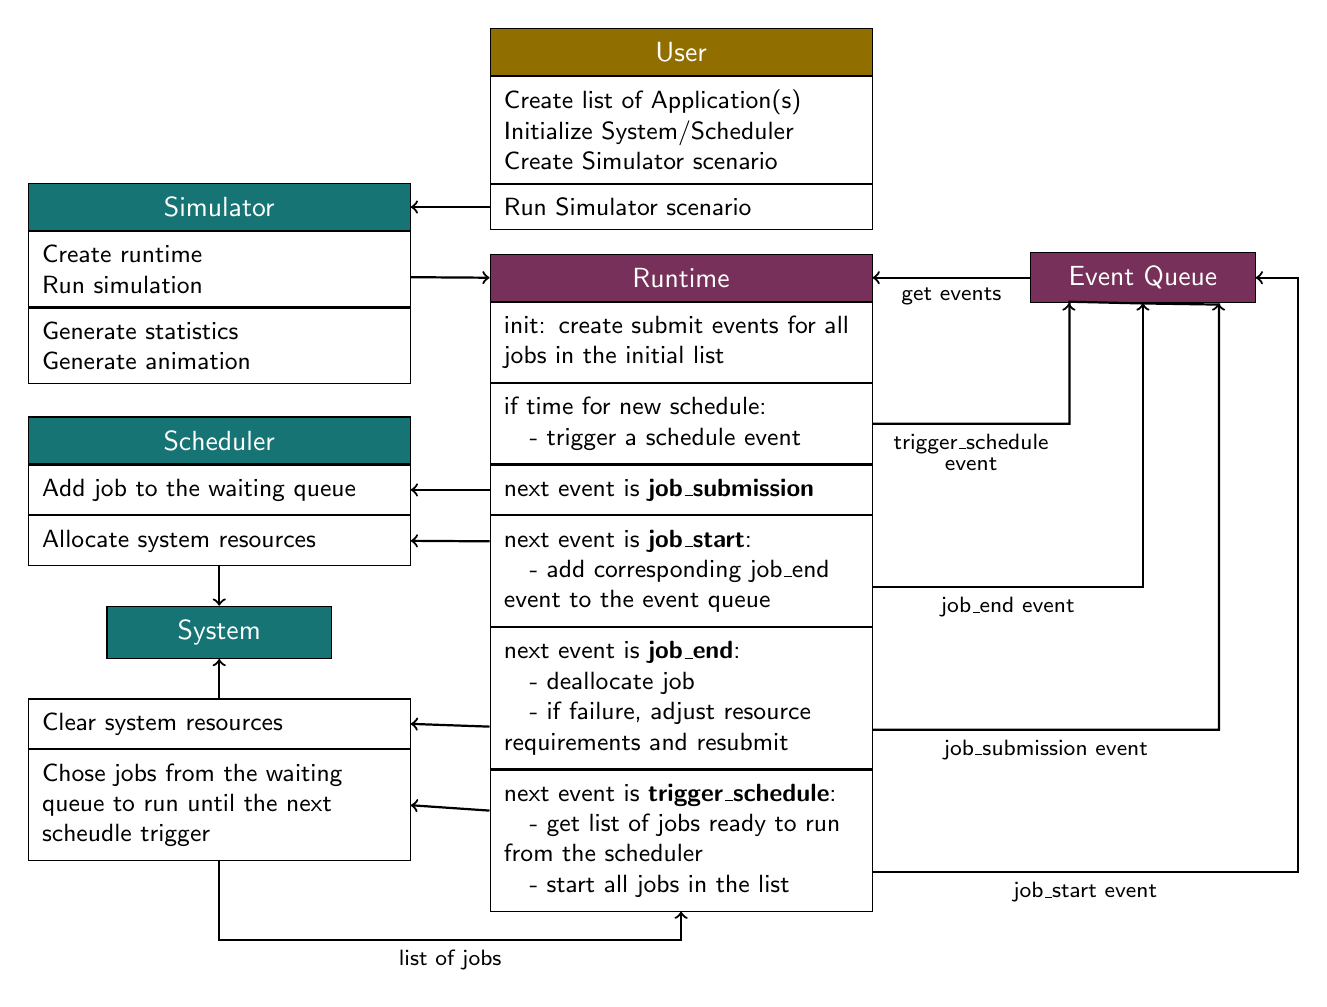
\begin{tikzpicture}
[node distance = 0.5cm, auto,font=\footnotesize,
% STYLES
every node/.style={node distance=3cm},
events/.style={font=\footnotesize\sffamily},
workflow/.style={rectangle, draw, inner sep= 5pt, text width=4.5cm, node distance=0.25cm, font=\small\sffamily},
internal/.style={rectangle, draw, fill={rgb:red,31;green,164;blue,163}, inner sep=5pt, text width=4.5cm, text badly centered, minimum height=0.2cm, text=white, font=\sffamily},
api/.style={rectangle, draw, fill={rgb:red,96;green,39;blue,73}, inner sep=5pt, text width=4.5cm, text badly centered, minimum height=0.2cm, text=white, font=\sffamily},
user/.style={rectangle, draw, fill={rgb:red,255;green,192;blue,0}, inner sep=5pt, text width=4.5cm, text badly centered, minimum height=0.2cm, text=white, font=\sffamily}]

% User
\node [user] (user) {User};
\node [workflow, below=0 of user] (user-desc) {Create list of Application(s)\\
Initialize System/Scheduler \\ Create Simulator scenario};
\node [workflow, below=0 of user-desc] (user-create) {Run Simulator scenario};

\node [internal, left=1cm of user-create] (runtime) {Simulator};
\node [workflow, below=0 of runtime] (runtime-init) {Create runtime\\Run simulation};
\node [workflow, below=0 of runtime-init] {Generate statistics\\Generate animation};

\node [api, below=0.3cm of user-create] (simulator) {Runtime};
\node [workflow, below=0 of simulator] (sim-init) {init: create submit events for all jobs in the initial list};
\node [workflow, below=0 of sim-init] (sim-trigger) {if time for new schedule:\\ \quad - trigger a schedule event};
\node [workflow, below=0 of sim-trigger] (sim-submission) {next event is \textbf{job\_submission}};
\node [workflow, below=0 of sim-submission] (sim-start) {next event is \textbf{job\_start}:\\ \quad - add corresponding job\_end event to the event queue};
\node [workflow, below=0 of sim-start] (sim-end) {next event is \textbf{job\_end}:\\ \quad - deallocate job \\ \quad - if failure, adjust resource requirements and resubmit};
\node [workflow, below=0 of sim-end] (sim-last) {next event is  \textbf{trigger\_schedule}:\\ \quad - get list of jobs ready to run from the scheduler\\ \quad - start all jobs in the list};

\node [api, right=2cm of simulator, text width=2.5cm] (eventq) {Event Queue};

\node [workflow, left=1cm of sim-submission] (sch-add) {Add job to the waiting queue};
\node [internal, above=0 of sch-add] (scheduler) {Scheduler};
\node [workflow, below=0 of sch-add] (sch-allocate) {Allocate system resources};

\node [internal, below=0.5cm of sch-allocate, text width=2.5cm] (system) {System};

\node [workflow, below=0.5cm of system] (sch-clear) {Clear system resources};
\node [workflow, below=0 of sch-clear] (sch-trigger) {Chose jobs from the waiting queue to run until the next scheudle trigger};

%%%%%%%%%%%%%%%%

\path[->,thick] 
(user-create) edge (runtime)
(eventq) edge node[events, auto] (evq) {get events} (simulator)
(sim-submission) edge (sch-add)
(sch-allocate) edge (system)
(sch-clear) edge (system);

\draw[->,thick] (runtime-init.east)+(0,-1mm) -- (simulator.west);

\draw[->,thick] (sim-trigger.east) -| node[events, pos=0.25,below] (tr_ev) {trigger\_schedule} ++(2.5,0) -- ++(0,1.55) -- (eventq.south)+(-9.4mm,0);	
\draw[->,thick] (sim-start.east)+(0,-2mm) -| node[events, pos=0.25,below] {job\_end event} (eventq.south);
\draw[->,thick] (sim-end.east)+(0,-4mm) -| node[events, pos=0.25,below] {job\_submission event} ++(4.4,0) -- ++(0,5) -- (eventq.south)+(9.6mm,0);
\draw[->,thick] (sim-last.east)+(0,-4mm) -| node[events, pos=0.25,below] {job\_start event} ++(5.4,0) -- ++(0,7)  |- (eventq.east);	

\draw[->,thick] (sim-start.west)+(0,3.8mm) -- (sch-allocate.east);
\draw[->,thick] (sim-end.west)+(0,-3.6mm) -- (sch-clear.east);
\draw[->,thick] (sim-last.west)+(0,3.8mm) -- (sch-trigger.east);

% list of jobs from scheduler to runtime
\draw[->,thick] (sch-trigger.south) |- ++(0,-1) -| node[events, pos=0.25,below] {list of jobs} (sim-last.south);

%%%%%%%%%%%

\node [events, below=-0.2cm of tr_ev] {event};


\end{tikzpicture} 
%\caption{ScheduleFlow Class Diagram}
%\label{fig:simulator}
%\end{figure}

\end{document}